\documentclass[compress]{beamer}

\usetheme{Singapore}
\usecolortheme{rose}
\usepackage{amsmath,amsfonts,amssymb}

\title{Sense Sentiment Similarity: An Analysis}
\author{Mitra Mohtarami et al.}
\institute{Presented by Shih-Ming Wang \\ NLPLab, Institute of Information Science, Academia Sinica}
\date{12-23-2015}
\subject{Computer Science}
\begin{document}
\beamertemplatenavigationsymbolsempty

\begin{frame}
 \maketitle
\end{frame}

\begin{frame}
	 \frametitle{Outline}
	 \tableofcontents
\end{frame}

\section{Introduction}
\begin{frame}{\secname}
\begin{itemize}
\item Word similarity - which similarity?
\item A brief History\footnote{\url{https://www.gavagai.se/blog/2015/09/30/a-brief-history-of-word-embeddings/}}
\item Distributional Semantic - represent a word by its context
\begin{itemize}
      \item Document as context - LSA, LDA\\
      learns semantic relatedness (e.g. ``boat'' $–-$ ``water'')
      \item Nearby words as context - \textit{word2vec}, PMI factorization\\
      learns semantic similarity (e.g. ``boat'' $–-$ ``ship'')
\end{itemize}
\item Not capturing accurate sentiment polarity?
\end{itemize}
\end{frame}

\section{Related Work}
\subsection{Topic Model}
\begin{frame}{\subsecname}
\begin{itemize}
\item Assume documents belong to some hidden topics, and each topic has different frequent words
\item Latent Semantic Analysis (LSA) - apply SVD to factor term-document co-occurrence matrix ($M=W\Sigma D^T$)
\item Latent Dirichlet Allocation (LDA) - Bayesian analysis on unigram model
\begin{itemize}
      \item Assume $k$ topics, each represented by $V$ dimension vector as distribution over vocabulary
      \item Each word represented by $k$ dimension vector as distribution over topics
\end{itemize}
\end{itemize}
\end{frame}

\subsection{Distributional Ccontext}
\begin{frame}{\subsecname}
\begin{itemize}
\item PMI factorization - apply SVD on word-word concurrence matrix ($M=W\Sigma C^T$)
\item skip-gram - optimizing the probability of the concurrence of a word and its nearby words
\item The two have been shown to be alike theoretically and empirically
\item For word similarity, distributional context is better than topic models
\end{itemize}
\end{frame}

\section[Sentiment Similarity]{Word Vector for Sentiment Similarity}
\begin{frame}[allowframebreaks]{\secname}
\begin{itemize}
\item Goal - measure sentiment similarity given two words $X, Y$
\item Methods
\begin{itemize}
\item Construct two d-dimensional vectors $\vec{X}, \vec{Y}$
\item Apply similarity function $Sim(X, Y)$, (cosine, correlation?)
\item Determine a threshold for $Sim$ (middle of the range of $S$?)
\end{itemize}
\item Solution
\begin{itemize}
\item Measure the relation of a word to  $12$ emotion categories
\item Apply correlation
$Sim(X,Y)=\sum\limits_{i=1}^d (\vec{X_i}-\bar{X})(\vec{Y_i}-\bar{Y})/(n-1)S_{\vec{X}} S_{\vec{Y}}$
\item Determine a threshold by considering synonyms, antonyms of $X, Y$
\end{itemize}
\end{itemize}

\framebreak

\begin{itemize}
\item \textbf{Step1} Build Vectors
\item Emotion categories:  anger, disgust, fear, guilt, sadness, shame, interest, joy, surprise, desire, love, courage
\item Select synonyms for each category as seeds
\begin{itemize}
\item Balance - Select equal amount of synonyms for each category
\item Relevant - Choose most similar synonyms according to semantic similarity scores computed by LSA
\end{itemize}
\item For a word X and a category $cat_k$ $\vec{X}_k=\sum\limits_{seed_i\in cat_k}coocur(X,seed_i)$
\item Problem: coocur is often $0$
\item Solution: $\vec{X}_k=\sum\limits_{W\in synset(X)}\sum\limits_{seed_i\in cat_k}coocur(W,seed_i)$
\end{itemize}

\framebreak

\begin{itemize}
\item \textbf{Step2} Similarity Function $Sim(X,Y)=corr(\vec{X}, \vec{Y})$
\item \textbf{Step3} Similarity Threshold
\item For two similar words X, Y, and their antonyms $\sim$X, $\sim$Y
\begin{itemize}
\item $Sim(\vec{X},\vec{Y})>Sim(\vec{X},\sim\vec{Y})$
\item $Sim(\vec{X},\vec{Y})>Sim(\sim\vec{X},\vec{Y})$
\end{itemize}
\item Threshold: $Max\{Sim(\vec{X},\sim\vec{Y}), Sim(\sim\vec{X},\vec{Y})\}$
\item With threshold $0$, define $Sim(X,Y) = corr(\vec{X},\vec{Y})-Max\{corr(\vec{X},\sim\vec{Y}), corr(\sim\vec{X},\vec{Y})\}$ 
\item Empirically better than taking $Sim(X,Y)=corr(\vec{X},\vec{Y})$
\end{itemize}
\end{frame}

\section{Experiments}
\subsection{Tasks}
\begin{frame}{\subsecname}
\begin{itemize}
\item  Indirect yes/no question answer pairs (IQAP) Inference
\begin{itemize}
\item $Sim(Adj_Q, Adj_A)>0$ leads to answer yes
\end{itemize}
\item  Sentiment Orientation Prediction 
\begin{itemize}
\item Pick 7 pwords and 7 nwords
\item polarity(w) = $\sum\limits_{p\in pwords}Sim(w,p)-\sum\limits_{p\in  nwords}Sim(w,n)$
\end{itemize}
\item Compare different similarity function PMI, LSA, proposed
\end{itemize}
\end{frame}

\subsection{Settings}
\begin{frame}{\subsecname}
\begin{itemize}
\item Training
\begin{itemize}
\item 50k movie reviews for calculating concurrence (PMI \& proposed)
\item TASA, 61k documents for LSA
\end{itemize}
\item Testing
\begin{itemize}
\item IQAP, 125 Question/Answer pairs
\item MPQA 4000 positive/negative words
\end{itemize}
\end{itemize}
\end{frame}

\subsection{Results}
\begin{frame}{\subsecname}
\begin{table}[]
\centering
\begin{tabular}{|c|c|c|c|}
\hline

Method   & Precision & Recall & F1    \\ \hline
PMI      & 60.61     & 58.70  & 59.64 \\ \hline
LSA      & 66.70     & 54.95  & 60.26 \\ \hline
Proposed & 75.03     & 77.85  & 76.41 \\ \hline
\end{tabular}
\caption{IQAP Results}
\end{table}
    
\begin{table}[]
\centering
\begin{tabular}{|c|c|c|c|}
\hline

Method   & Precision & Recall & F1    \\ \hline
PMI      & 56.20     & 56.36  & 55.01 \\ \hline
LSA      & 66.31     & 66.89  & 66.26 \\ \hline
Proposed & 73.07     & 73.89  & 73.11 \\ \hline
\end{tabular}
\caption{Sentiment Polarity Results}
\end{table}
\end{frame}

\subsection{Error Analysis}
\begin{frame}[allowframebreaks]{\subsecname}


\begin{itemize}
\item Noise in emotion categories?
\begin{itemize}
\item Apply SVD on word-category matrix ($|V|x12$)
\item 11 dimension achieves best F1 on sentiment polarity task
\end{itemize}
\item Balance and relevance
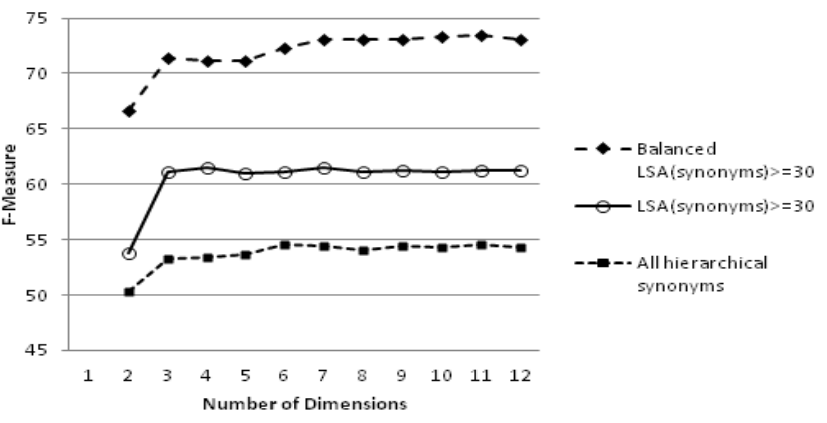
\includegraphics[height=4cm]{error.png}
\end{itemize}
\framebreak

\begin{itemize}
\item Role of synonyms and antonyms
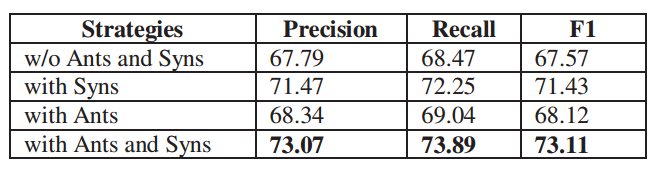
\includegraphics[width=10cm]{error2.png}
\end{itemize}
\end{frame}

\section{Conclusion}
\begin{frame}{\secname}
\begin{itemize}
\item A method to construct word vector from prior knowledge is proposed
\item Correlation is used to measure sentiment similarity for words
\item Outperforms baselines on two tasks
\end{itemize}
\end{frame}


\end{document}
